\documentclass[11pt]{article}

\usepackage[a4paper,margin=1in]{geometry}
\usepackage{amsmath,amssymb,amsthm,mathtools}
\usepackage{enumitem}
\usepackage{hyperref}
\usepackage[table]{xcolor}
\usepackage{booktabs}
\usepackage{array}
\usepackage{graphicx}
\usepackage{pgfplots}
\pgfplotsset{compat=1.18}

\hypersetup{
	colorlinks=true,
	linkcolor=blue,
	urlcolor=blue,
	citecolor=blue
}

\newcommand{\F}{\mathbb{F}}
\newcommand{\GL}{\operatorname{GL}}
\newcommand{\Mat}{\operatorname{Mat}}

\begin{document}
	
	\section{\texorpdfstring{Tables and graphs for \(\lvert GL_m(\F_q)\rvert/\lvert \Mat_m(\F_q)\rvert\)}{Tables and graphs for |GL_m(F_q)|/|Mat_m(F_q)|}}
	
	Recall that
	\[
	|\Mat_m(\F_q)|=q^{m^2},
	\qquad
	|GL_m(\F_q)|=\prod_{i=0}^{m-1}(q^m-q^i),
	\]
	and hence
	\[
	\frac{|GL_m(\F_q)|}{|\Mat_m(\F_q)|}
	=
	\prod_{j=1}^{m}(1-q^{-j}).
	\]
	
	\subsection{\texorpdfstring{Symbolic table for \(|\Mat_m(\F_q)|\), \(|GL_m(\F_q)|\), and the ratio}{Symbolic table}}
	
	\begin{center}
		\resizebox{\textwidth}{!}{%
			\renewcommand{\arraystretch}{1.35}
			\begin{tabular}{c c c c}
				\toprule
				\rowcolor{blue!15}
				\(m\) & \(\lvert \Mat_m(\F_q)\rvert\) & \(\lvert GL_m(\F_q)\rvert\) & \(\dfrac{\lvert GL_m(\F_q)\rvert}{\lvert \Mat_m(\F_q)\rvert}\) \\
				\midrule
				\(1\) & \(q\) & \(q-1\) & \(1-q^{-1}\) \\
				
				\rowcolor{gray!8}
				\(2\) & \(q^4\) & \((q^2-1)(q^2-q)\) & \((1-q^{-1})(1-q^{-2})\) \\
				
				\(3\) & \(q^9\) & \((q^3-1)(q^3-q)(q^3-q^2)\) & \((1-q^{-1})(1-q^{-2})(1-q^{-3})\) \\
				
				\rowcolor{gray!8}
				\(4\) & \(q^{16}\) & \((q^4-1)(q^4-q)(q^4-q^2)(q^4-q^3)\) & \((1-q^{-1})(1-q^{-2})(1-q^{-3})(1-q^{-4})\) \\
				
				\(5\) & \(q^{25}\) & \((q^5-1)(q^5-q)(q^5-q^2)(q^5-q^3)(q^5-q^4)\) & \(\prod_{j=1}^{5}(1-q^{-j})\) \\
				
				\rowcolor{gray!8}
				\(\vdots\) & \(\vdots\) & \(\vdots\) & \(\vdots\) \\
				
				\(m\) & \(q^{m^2}\) & \(\displaystyle\prod_{i=0}^{m-1}(q^m-q^i)\) & \(\displaystyle\prod_{j=1}^{m}(1-q^{-j})\) \\
				\bottomrule
			\end{tabular}%
		}
	\end{center}
	
	\subsection{\texorpdfstring{Numerical table for \(q=2\)}{Numerical table for q=2}}
	
	For \(q=2\), we have
	\[
	|\Mat_m(\F_2)|=2^{m^2},
	\qquad
	\frac{|GL_m(\F_2)|}{|\Mat_m(\F_2)|}
	=
	\prod_{j=1}^{m}(1-2^{-j}).
	\]
	
	\begin{center}
		\renewcommand{\arraystretch}{1.35}
		\begin{tabular}{c c c c}
			\toprule
			\rowcolor{red!15}
			\(m\) & \(\lvert \Mat_m(\F_2)\rvert\) & \(\lvert GL_m(\F_2)\rvert\) & \(\dfrac{\lvert GL_m(\F_2)\rvert}{\lvert \Mat_m(\F_2)\rvert}\) \\
			\midrule
			\(1\) & \(2\) & \(1\) & \(0.500000\) \\
			
			\rowcolor{gray!8}
			\(2\) & \(16\) & \(6\) & \(0.375000\) \\
			
			\(3\) & \(512\) & \(168\) & \(0.328125\) \\
			
			\rowcolor{gray!8}
			\(4\) & \(65536\) & \(20160\) & \(0.307617\) \\
			
			\(5\) & \(33554432\) & \(9999360\) & \(0.298004\) \\
			
			\rowcolor{gray!8}
			\(6\) & \(68719476736\) & \(20158709760\) & \(0.293348\) \\
			\bottomrule
		\end{tabular}
	\end{center}
	
	\subsection{\texorpdfstring{Colorful graph of \(\lvert GL_m(\F_q)\rvert/\lvert \Mat_m(\F_q)\rvert\)}{Colorful graph of the ratio}}
	
	The following graph shows
	\[
	y=\frac{|GL_m(\F_q)|}{|\Mat_m(\F_q)|}
	=
	\prod_{j=1}^{m}(1-q^{-j})
	\]
	as a function of \(m\), for \(q=2,3,5\).
	
	\begin{center}
		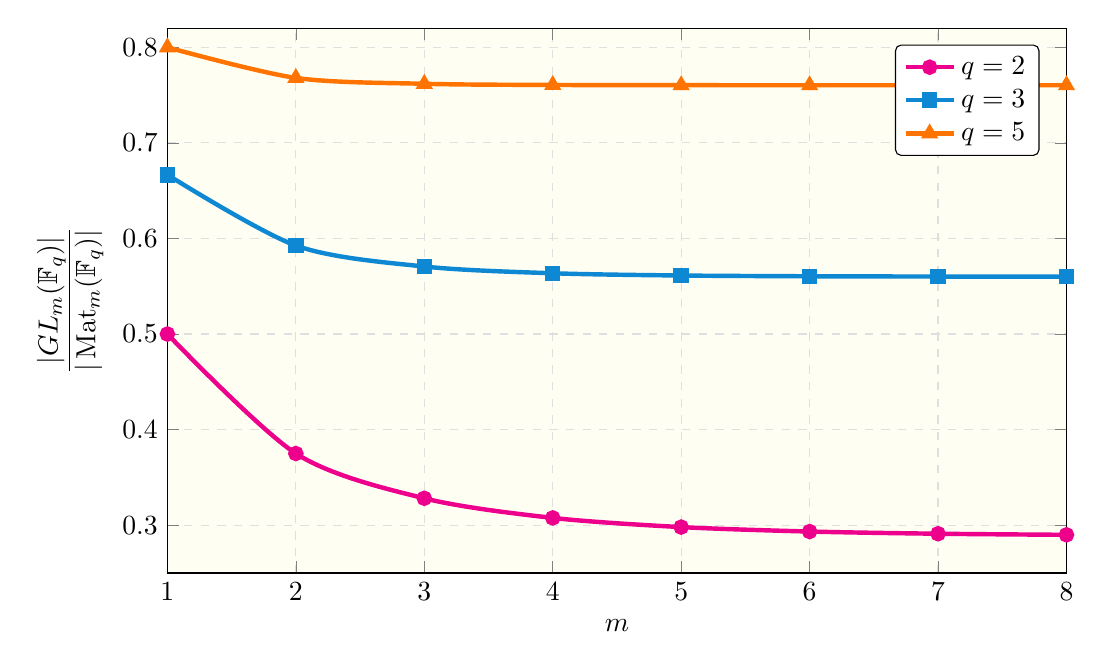
\begin{tikzpicture}
			\begin{axis}[
				width=13cm,
				height=8.5cm,
				xlabel={$m$},
				ylabel={$\dfrac{|GL_m(\F_q)|}{|\Mat_m(\F_q)|}$},
				xmin=1, xmax=8,
				ymin=0.25, ymax=0.82,
				xtick={1,2,3,4,5,6,7,8},
				ymajorgrids=true,
				xmajorgrids=true,
				grid style={dashed, gray!25},
				axis background/.style={fill=yellow!5},
				legend style={
					at={(0.97,0.97)},
					anchor=north east,
					draw=black,
					fill=white,
					rounded corners=2pt
				},
				every axis plot/.append style={ultra thick}
				]
				
				\addplot[
				color=magenta,
				mark=*,
				mark options={fill=magenta},
				smooth
				] coordinates {
					(1,0.5)
					(2,0.375)
					(3,0.328125)
					(4,0.3076171875)
					(5,0.298004150390625)
					(6,0.2933478355407715)
					(7,0.2910560965538025)
					(8,0.2899184823036194)
				};
				\addlegendentry{$q=2$}
				
				\addplot[
				color=cyan!70!blue,
				mark=square*,
				mark options={fill=cyan!70!blue},
				smooth
				] coordinates {
					(1,0.6666666667)
					(2,0.5925925926)
					(3,0.5706447188)
					(4,0.5635989238)
					(5,0.5612511784)
					(6,0.5604553718)
					(7,0.5601834231)
					(8,0.5600901142)
				};
				\addlegendentry{$q=3$}
				
				\addplot[
				color=orange!90!red,
				mark=triangle*,
				mark options={fill=orange!90!red},
				smooth
				] coordinates {
					(1,0.8)
					(2,0.768)
					(3,0.761856)
					(4,0.7606370304)
					(5,0.7603930061)
					(6,0.7603442021)
					(7,0.7603344414)
					(8,0.7603324892)
				};
				\addlegendentry{$q=5$}
				
			\end{axis}
		\end{tikzpicture}
	\end{center}


	
\end{document}